% IEEE Conference Template
% IF3211 Domain-Specific Computation -- Kelompok 07
% Kompilasi: pdflatex main && bibtex main && pdflatex main && pdflatex main
\documentclass[conference]{IEEEtran}
\IEEEoverridecommandlockouts

\usepackage[T1]{fontenc}
\usepackage[utf8]{inputenc}
\usepackage{cite}
\usepackage{amsmath,amssymb,amsfonts}
\usepackage{graphicx}
\usepackage{textcomp}
\usepackage{xcolor}
\usepackage{url}
\usepackage{booktabs}
\usepackage{hyperref}
\usepackage{tikz}
\usetikzlibrary{positioning,arrows.meta,shapes.geometric,fit}

\graphicspath{{./images/}{images/}}

\def\BibTeX{{\rm B\kern-.05em{\sc i\kern-.025em b}\kern-.08em
    T\kern-.1667em\lower.7ex\hbox{E}\kern-.125emX}}

\begin{document}

\title{MacroPlus: Sistem Komputasi Pendukung Keputusan Nutrisi---Integrasi Pemodelan Metabolik, ILP \textit{Multi-Objective}, Perencanaan Menu, dan Pemantauan Kepatuhan Longitudinal%
\thanks{Tugas Besar IF3211 \emph{Domain-Specific Computation} -- Kelompok 07, Program Studi Sistem dan Teknologi Informasi, Institut Teknologi Bandung.}}

% --- 2x2 author grid (IEEE conference-compatible) ---
\author{%
\begin{tabular}{cc}
\IEEEauthorblockN{Muhammad Adam Mirza} & \IEEEauthorblockN{Devon Wiraditya Tanumihardja} \\
\IEEEauthorblockA{\textit{18223015} \\ Institut Teknologi Bandung} &
\IEEEauthorblockA{\textit{18223039} \\ Institut Teknologi Bandung} \\[1.0ex]
\IEEEauthorblockN{Muhammad Aqmar Fayyaz Zakaria} & \IEEEauthorblockN{Catherine Alicia Putri} \\
\IEEEauthorblockA{\textit{18223043} \\ Institut Teknologi Bandung} &
\IEEEauthorblockA{\textit{18223069} \\ Institut Teknologi Bandung}
\end{tabular}}

\maketitle

\begin{abstract}
Aplikasi penghitung kalori konvensional umumnya hanya berfungsi sebagai pencatat makanan (\textit{food logger}) tanpa analisis biologis komprehensif, optimasi terhadap kebutuhan metabolik individu, perencanaan menu otomatis, maupun pemantauan kepatuhan nutrisi jangka panjang. Penelitian ini mengembangkan \textbf{MacroPlus}, sistem komputasi berbasis web yang mengintegrasikan lima lapisan: (1) penghitungan kebutuhan energi (BMR \textit{Mifflin--St Jeor} dan TDEE dengan \textit{activity multiplier} ACSM); (2) target makronutrien berdasarkan AMDR \textit{Institute of Medicine}; (3) rekomendasi makanan \textit{multi-objective} melalui \textit{Integer Linear Programming} (ILP) dengan solver CBC via PuLP; (4) perencanaan menu mingguan per-slot waktu makan yang menghasilkan agregasi daftar belanja; dan (5) pemantauan kepatuhan longitudinal melalui skor harian, \textit{Nutrition Adherence Score} (NAS), serta pencatatan berat badan. Sistem diimplementasikan menggunakan FastAPI--Firestore pada sisi \textit{backend} dan React--TypeScript--Recharts pada sisi \textit{frontend} dengan autentikasi JWT. Validasi pada studi kasus pria 22 tahun (68~kg, 172~cm, \textit{moderate}, \textit{muscle gain}) menunjukkan solver mencapai status \textit{Optimal} dengan total deviasi mendekati nol terhadap target 2813~kcal, 176~g protein, 352~g karbohidrat, 78~g lemak. Modul perencanaan menu menghasilkan tujuh hari menu lengkap dalam waktu sub-detik per hari, sedangkan modul progres menghitung NAS dan tren makro--kalori secara konsisten. MacroPlus memposisikan diri sebagai \textit{decision support system} nutrisi yang ilmiah, dapat direplikasi, dan terintegrasi secara penuh dari input biologis hingga rekomendasi belanja.
\end{abstract}

\begin{IEEEkeywords}
makronutrien, Mifflin--St Jeor, TDEE, AMDR, \textit{integer linear programming}, perencanaan menu, kepatuhan nutrisi, \textit{domain-specific computation}
\end{IEEEkeywords}

\section{Pendahuluan}

\subsection{Latar Belakang}
Kebutuhan energi dan makronutrien (karbohidrat, protein, lemak) merupakan aspek fundamental metabolisme manusia; ketidakseimbangannya berkontribusi pada obesitas, sarkopenia, dan beragam penyakit metabolik kronis~\cite{hall2011quantification}. Pemodelan kebutuhan energi individu yang akurat menjadi prasyarat penting bagi setiap intervensi nutrisi yang rasional~\cite{frankenfield2005comparison}. Saat ini banyak aplikasi penghitung kalori membantu pengguna mencatat asupan, namun mayoritas berperan sebagai \textit{food logger} tanpa analisis biologis komprehensif, optimasi formal, perencanaan menu, atau pemantauan kepatuhan jangka panjang.

\subsection{Tinjauan Pustaka}
Aplikasi seperti MyFitnessPal, Cronometer, dan MacroFactor memiliki basis data luas tetapi rekomendasinya umumnya heuristik dan bukan optimasi formal. Pendekatan optimasi diet sebenarnya telah dirumuskan sejak Stigler~\cite{stigler1945cost}, kemudian diperluas menjadi \textit{Integer Linear Programming} untuk menangani keputusan diskret~\cite{wolsey1998integer}. Survei terbaru terhadap \textit{food recommender system}~\cite{tran2018overview} menyoroti perlunya integrasi antara model nutrisi formal dan algoritma rekomendasi. Distribusi makro tingkat populasi telah diatur AMDR \textit{Institute of Medicine}~\cite{iom2005}, dan pola tiga waktu makan plus camilan diadopsi oleh USDA \textit{Dietary Guidelines}~\cite{usda_dgaa}.

\subsection{Rumusan Masalah dan Tujuan}
Empat pertanyaan penelitian dijawab: (1) Bagaimana kebutuhan energi dimodelkan dari parameter biologis tervalidasi? (2) Bagaimana ILP memenuhi target nutrisi secara simultan? (3) Bagaimana model dan optimasi tersebut diperluas menjadi perencanaan menu mingguan + daftar belanja? (4) Bagaimana kepatuhan jangka panjang diukur secara kuantitatif dan dapat ditafsirkan?

\subsection{Kontribusi}
Kontribusi MacroPlus ada empat: (i) integrasi BMR/TDEE/AMDR/ILP dalam satu pipeline; (ii) perencanaan menu mingguan berbasis ILP per-slot waktu makan, dengan agregasi daftar belanja yang biasanya hilang di aplikasi populer; (iii) \textit{Nutrition Adherence Score} (NAS) sebagai metrik komposit kepatuhan yang transparan; (iv) implementasi referensi sebagai SaaS dengan autentikasi JWT, sehingga dapat direplikasi dan diuji ulang.

\section{Metode}

\subsection{Arsitektur Sistem}
Sistem terdiri dari \textit{backend} FastAPI yang memuat sembilan \textit{router} (autentikasi, pengguna, makanan, log harian, analisis, optimasi, perencanaan menu, daftar belanja, progres) serta \textit{frontend} React/TypeScript. Persistensi menggunakan Cloud Firestore (model dokumen) sebagai pengganti basis data relasional klasik, dengan koleksi: \texttt{users}, \texttt{foods}, \texttt{users/\{uid\}/logs/\{date\}/items}, \texttt{users/\{uid\}/meal\_plans/\{date\}}, dan \texttt{users/\{uid\}/weight\_logs}. Autentikasi memakai JWT HS256 berusia tujuh hari~\cite{jones2007jwt} dengan \textit{password hashing} bcrypt; pada sisi klien token disimpan di \texttt{localStorage} dan disuntikkan oleh \textit{axios interceptor}.

\begin{figure}[t]
  \centering
  \includegraphics[width=\columnwidth]{arsitektur.png}
  \caption{Arsitektur sistem MacroPlus---antarmuka, REST API, layanan optimasi, dan basis data dokumen.}
  \label{fig:arsitektur}
\end{figure}

\subsection{Diagram Alur Komputasi}
Gambar~\ref{fig:flow} merangkum alur dari masukan pengguna hingga keluaran rekomendasi, perencanaan, dan pemantauan.

\begin{figure}[t]
\centering
\begin{tikzpicture}[node distance=4.2mm, font=\scriptsize,
  every node/.style={align=center, rounded corners, draw=black!70,
                     minimum height=4.4mm, inner sep=2pt},
  proc/.style ={fill=blue!6, minimum width=20mm},
  data/.style ={fill=green!8, minimum width=20mm, shape=cylinder, shape border rotate=90, aspect=0.2},
  out/.style  ={fill=orange!10, minimum width=22mm},
  ->,>={Latex[length=1.4mm]}]
  \node[data] (u) {User Input\\(age, sex, $W$, $H$, activity, goal)};
  \node[proc, below=of u] (bmr) {BMR (Mifflin--St Jeor)};
  \node[proc, below=of bmr] (tdee) {TDEE = BMR $\times\,\alpha$};
  \node[proc, below=of tdee] (amdr) {Macro targets (AMDR)};
  \node[data, below=of amdr] (log) {Food log\\(daily items)};
  \node[proc, below=of log] (anal) {Nutritional analysis};
  \node[out,  right=10mm of anal] (opt) {ILP optimiser\\(single-slot recs)};
  \node[out,  above=of opt] (mp) {Meal planner\\(per-slot ILP $\times$ 7d)};
  \node[out,  above=of mp]  (gr) {Grocery list\\(aggregation)};
  \node[out,  below=of opt] (prog) {Progress\\(compliance, NAS, weight)};
  \draw (u)--(bmr); \draw (bmr)--(tdee); \draw (tdee)--(amdr); \draw (amdr)--(log);
  \draw (log)--(anal); \draw (anal)--(opt); \draw (opt)--(mp); \draw (mp)--(gr);
  \draw (anal.east) -- ++(0.45,0) |- (prog.west);
\end{tikzpicture}
\caption{Diagram alur komputasi MacroPlus: dari parameter biologis hingga lima keluaran (analisis, rekomendasi, perencanaan, daftar belanja, progres).}
\label{fig:flow}
\end{figure}

\subsection{Dataset Makanan}
Dataset terdiri atas 48 bahan pangan yang nilainya diselaraskan dengan Panganku Indonesia~\cite{panganku} dan USDA FoodData Central~\cite{usda_fdc}, dikelompokkan ke tujuh kategori. Tiap entri menyimpan kalori, protein, lemak, dan karbohidrat per 100~g.

\subsection{Perhitungan Metabolik dan AMDR}
Persamaan \textit{Mifflin--St Jeor}~\cite{mifflin1990new} dipilih karena lebih akurat untuk populasi modern~\cite{frankenfield2005comparison}:
\begin{align}
\text{BMR}_{\text{m}} &= 10W + 6{,}25H - 5A + 5 \\
\text{BMR}_{\text{f}} &= 10W + 6{,}25H - 5A - 161
\end{align}
TDEE dihitung dengan \textit{activity multiplier} ACSM~\cite{acsm2018,thomas2016position}:
\begin{equation}
\text{TDEE} = \text{BMR}\times\alpha,\quad \alpha\in\{1{,}2;\,1{,}375;\,1{,}55;\,1{,}725;\,1{,}9\}.
\end{equation}
Target kalori harian disesuaikan terhadap tujuan: $T_K = \text{TDEE}\times(1+\delta)$ dengan $\delta\in\{-0{,}15;\,0;\,+0{,}10\}$~\cite{thomas2016position,rodriguez2009position}. Target gram tiap makro diturunkan dari $T_K$ melalui titik tengah AMDR~\cite{iom2005}: $T_X = T_K\,s_X/e_X$ dengan $s=(0{,}50;\,0{,}25;\,0{,}25)$ dan $e=(4;\,4;\,9)$~kcal/g.

\subsection{Analisis Kualitas Nutrisi}
Tiga indikator dihitung: \textit{protein density} $\rho_P = P/K$, \textit{energy density} $\rho_E = K/m$~\cite{rolls2009dietary}, dan \textit{macro balance score}
\begin{equation}
\text{MBS} = \Bigl(1 - \tfrac{1}{2}\textstyle\sum_X |\hat{s}_X - s_X^{\star}|\Bigr)\times 100,
\end{equation}
dengan $s^{\star}=(0{,}55;\,0{,}225;\,0{,}275)$ (titik tengah AMDR). Deteksi defisiensi memakai ambang heuristik: $\pm10$~g protein, $\pm 40$--$50$~g karbohidrat, $+15$~g lemak, dan $\pm 300$~kcal.

\subsection{Formulasi ILP \textit{Multi-Objective}}
Pendekatan \textit{greedy} sering melanggar batas kalori atau lemak. ILP menjamin optimalitas terhadap beberapa target sekaligus~\cite{wolsey1998integer}. Untuk himpunan makanan $F$, $x_i\in\mathbb{Z}_{\ge0}$ menyatakan jumlah satuan $s=10$~g; $y_i\in\{0,1\}$ menandai apakah makanan $i$ dipilih; $e_K,e_P,e_C,e_F\ge0$ adalah deviasi absolut. Defisit didefinisikan $\Delta_X = \max(0, T_X - I_X)$. Fungsi tujuan dengan bobot prioritas protein:
\begin{equation}
\min\; 4\,e_P + 1{,}5\,e_C + 2\,e_F + 1\,e_K.
\end{equation}
Kendala linierisasi: $e_X \ge \Delta_X - \sum_i \tilde{x}_i$ dan $e_X \ge \sum_i \tilde{x}_i - \Delta_X$. Anggaran nutrisi:
\begin{align}
\sum_{i\in F}\tilde{c}_i x_i &\le 1{,}05\,\Delta_K + 50, \\
\sum_{i\in F}\tilde{f}_i x_i &\le 1{,}05\,\Delta_F + 5, \\
\sum_{i\in F}\tilde{p}_i x_i &\ge 0{,}5\,\Delta_P\;\;\text{jika } \Delta_P>5.
\end{align}
Kendala penghubung dan sparsitas: $x_i\le U y_i$, $x_i\ge y_i$, dan $1\le\sum_i y_i\le N_{\max}{=}4$. Model diselesaikan menggunakan CBC~\cite{forrest2005cbc} via PuLP~\cite{mitchell2011pulp} dengan batas waktu 10~detik.

\subsection{Perencanaan Menu Mingguan}
Modul perencana memecah hari menjadi empat \textit{slot} dengan distribusi default sarapan 25\%, makan siang 35\%, makan malam 30\%, dan camilan 10\%~\cite{usda_dgaa}. Untuk setiap \textit{slot} $m$, target slot dihitung $T_X^{(m)} = T_X\times\sigma_m$ dengan $\sigma_m$ pangsa \textit{slot}. ILP dijalankan terpisah per \textit{slot} dengan asupan saat ini nol dan dengan \textit{pool} makanan yang difilter berdasarkan kelayakan kategori untuk \textit{slot} tersebut (mis. sarapan menerima karbohidrat, buah, susu \& olahan, protein hewani/nabati). Hasil tujuh hari dipersist ke koleksi \texttt{meal\_plans}; permintaan ulang membaca data tersimpan. Pengguna dapat mengubah $\sigma$ selama $\sum_m\sigma_m=1$.

\subsection{Agregasi Daftar Belanja}
Daftar belanja dihasilkan dengan menjumlahkan gram tiap makanan dari seluruh \textit{slot} pada jendela tujuh hari, mengonversi makanan kategori buah/telur menjadi satuan butir berdasarkan tabel ukuran rumah tangga FAO yang dijadikan parameter di \texttt{PIECE\_FOODS}. Algoritmanya:
\begin{equation}
\Gamma_i = \sum_{d=1}^{7}\sum_{m\in M} g_{i,d,m},\quad
\pi_i =
\begin{cases}
\lceil \Gamma_i / p_i \rceil & \text{jika } i\in P,\\
- & \text{lainnya},
\end{cases}
\end{equation}
dengan $g_{i,d,m}$ gram makanan $i$ pada hari $d$ \textit{slot} $m$, $P$ himpunan makanan berbasis satuan, dan $p_i$ gram per butir.

\subsection{Analisis Kepatuhan Nutrisi}
Kepatuhan harian dihitung sebagai galat persentase rata-rata terhadap target,
\begin{equation}
\text{Score}_{X}(d) = \max(0,\,100 - \%\text{err}_X(d)),
\end{equation}
dengan $\%\text{err}_X(d) = |I_X(d) - T_X|/T_X\times100$. Skor harian gabungan adalah rerata empat makro. Untuk jendela $n$ hari, skor per makro adalah rata-rata $\%\text{err}_X$ dibalik 100. \textit{Nutrition Adherence Score} (NAS) didefinisikan
\begin{equation}
\text{NAS} = 0{,}4\,S_K + 0{,}3\,S_P + 0{,}2\,S_C + 0{,}1\,S_F,
\end{equation}
dengan klasifikasi \textit{Poor}/\textit{Fair}/\textit{Good}/\textit{Excellent} pada ambang $50/70/85$. Bobot mengutamakan kalori karena merupakan prediktor utama berat badan~\cite{hall2011quantification}, lalu protein karena substrat anabolik utama~\cite{thomas2016position,rodriguez2009position}; karbohidrat dan lemak memperoleh bobot lebih rendah karena AMDR mentolerir rentang yang lebih lebar~\cite{iom2005}. NAS adalah \emph{metrik turunan} yang \emph{diusulkan} oleh proyek ini dan dinyatakan eksplisit, bukan diambil verbatim dari literatur tunggal.

\subsection{Pemantauan Berat dan Keseimbangan Energi}
Berat dicatat ke koleksi \texttt{weight\_logs} dan otomatis memperbarui dokumen pengguna sehingga BMR/TDEE/target di-rekomputasi pada analisis hari berikutnya. Keseimbangan energi mengikuti kerangka Hall~\cite{hall2011quantification}: $\text{EB}(d) = I_K(d) - T_K$, dengan nilai negatif berarti defisit dan positif berarti surplus.

\subsection{Reprodusibilitas}
Implementasi lengkap dan dokumentasi (\textsc{readme}, laporan validasi ilmiah, audit kode--makalah, penilaian IF3211) tersedia di:
\begin{center}\small
\url{https://github.com/aqmarfayyaz/IF3050_Tugas-Besar_Kel07_Sistem-Analisis-dan-Optimasi-Asupan-Makronutrien}
\end{center}

\section{Hasil dan Diskusi}

\subsection{Implementasi Sistem}
Sistem terdiri atas 31 \textit{endpoint} REST dalam sembilan \textit{router} dan tujuh halaman rute pada \textit{frontend} (Landing, Login, Register, \textit{Profile Setup}, Dashboard, Food Logger, Analytics, Recommendations, Meal Planner, Progress, Settings). Dasbor utama (Gambar~\ref{fig:dashboard}) menampilkan progres kalori, empat \textit{stat card} makro, tren mingguan, dan kartu \textit{insight}. \textit{Food Logger} dan \textit{Analytics} memuat pencarian, filter, dan \textit{donut/radar chart} kualitas.

\begin{figure}[t]
  \centering
  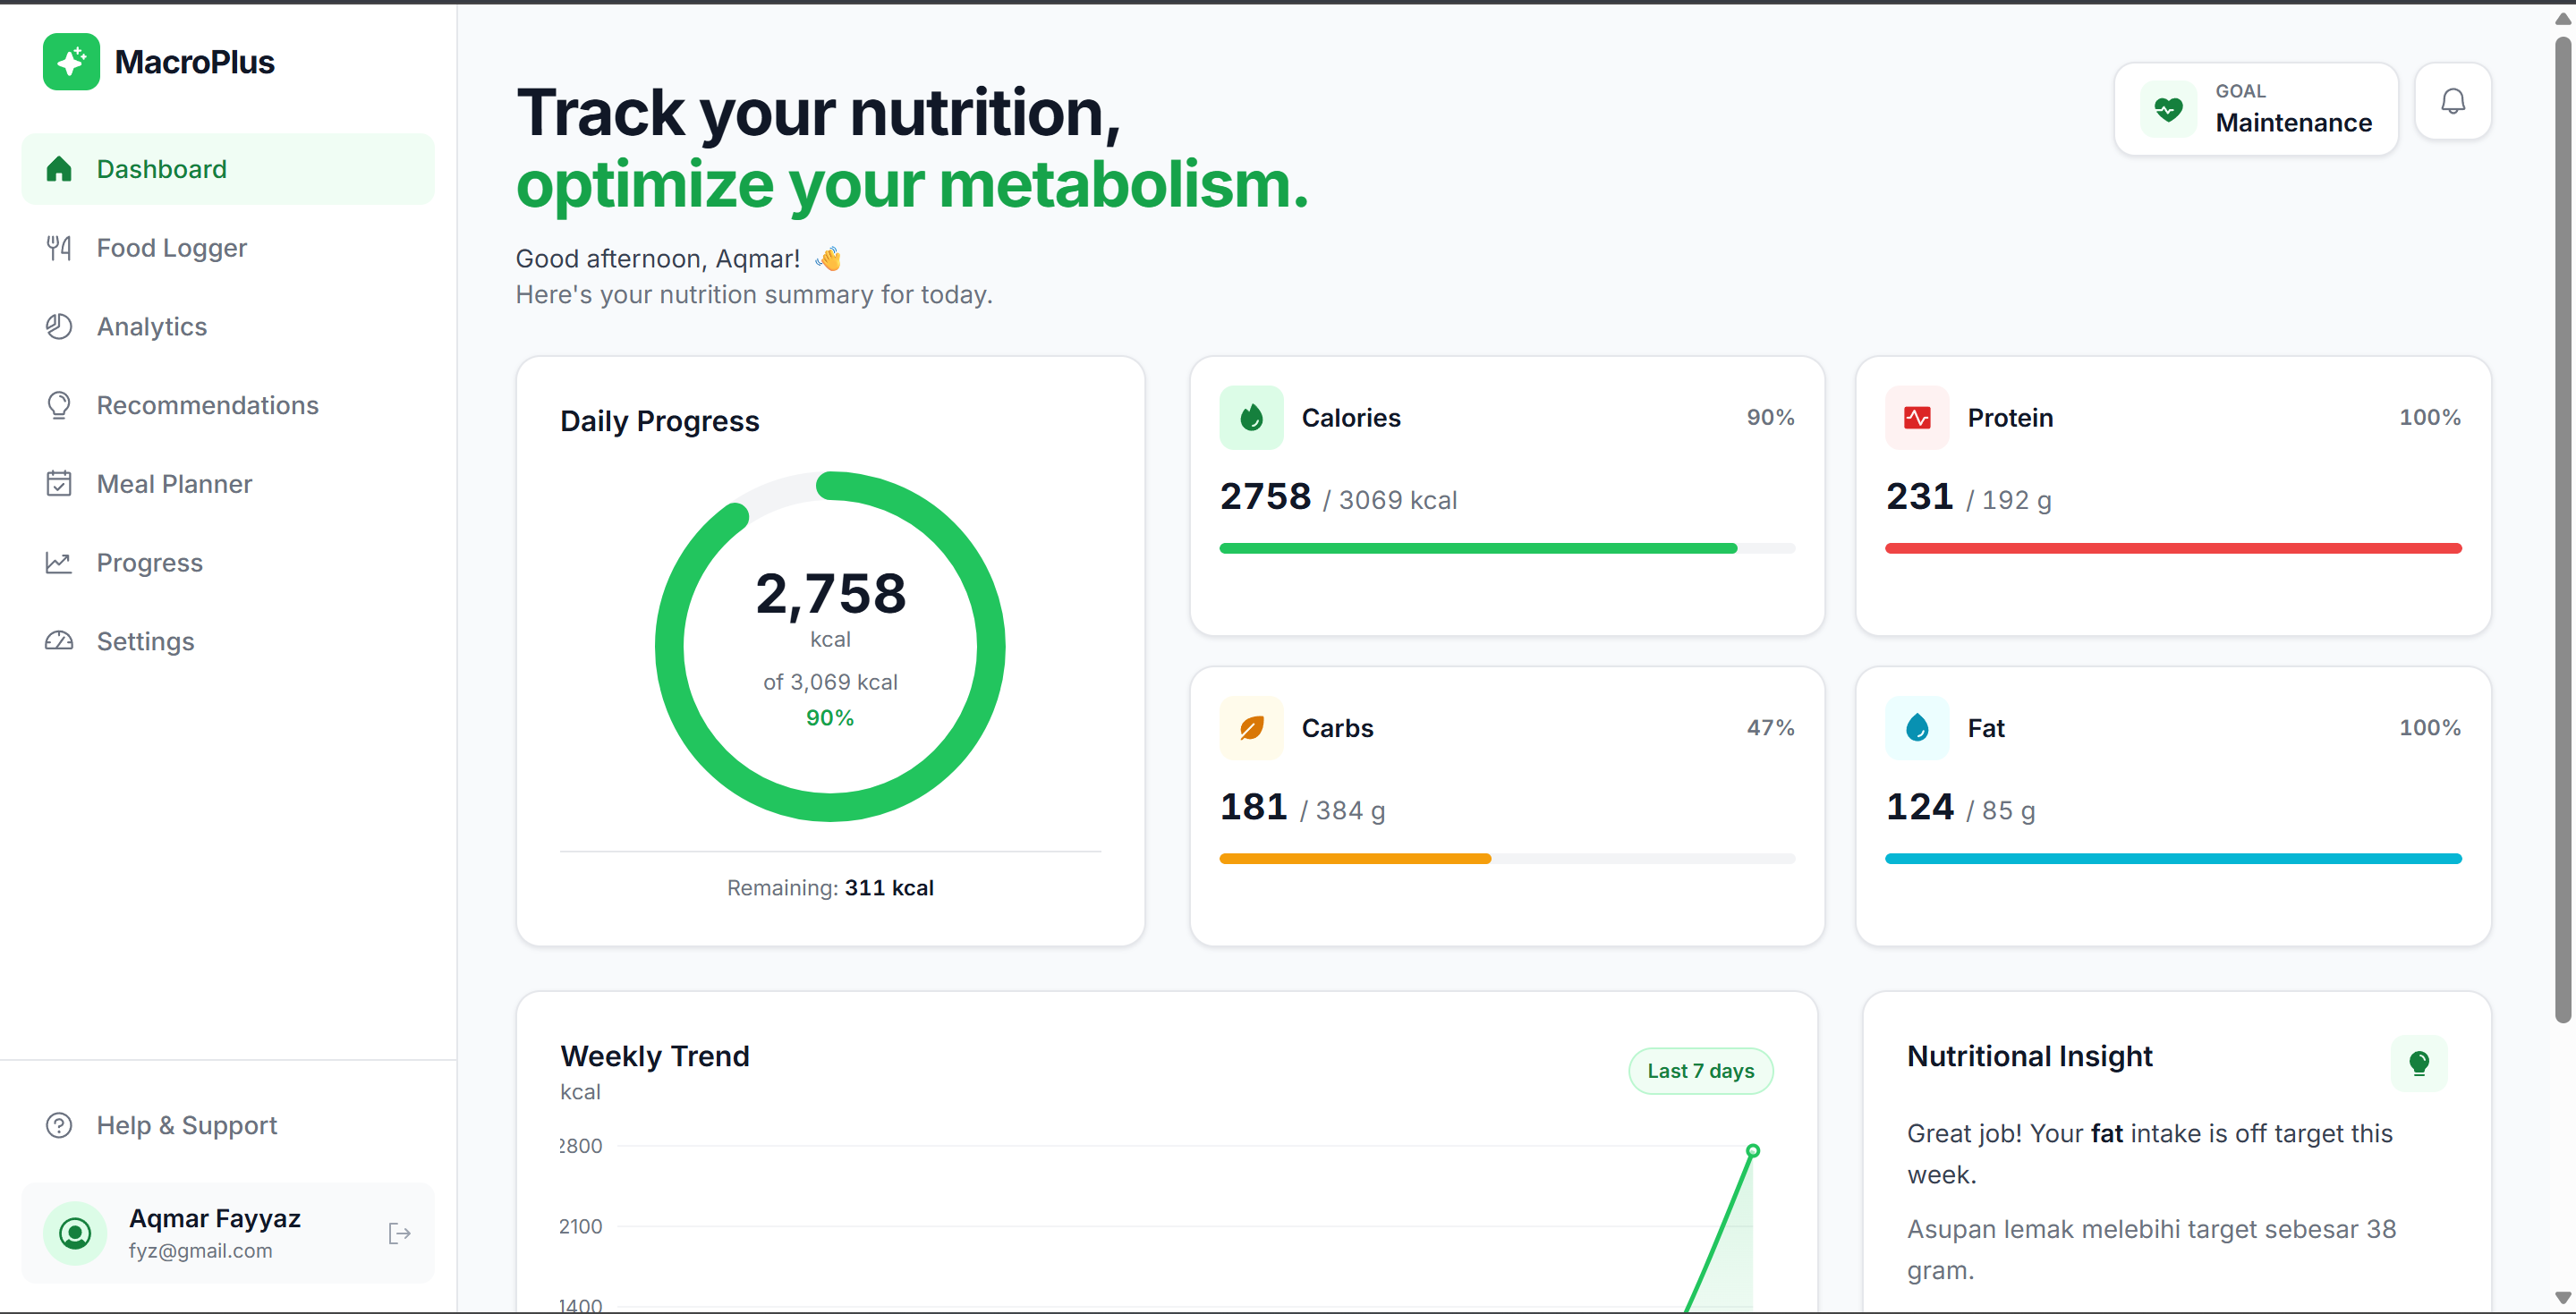
\includegraphics[width=\columnwidth]{dashboard.png}
  \caption{Dasbor utama: progres kalori, empat \textit{stat} makro, tren mingguan, dan \textit{insight}.}
  \label{fig:dashboard}
\end{figure}

\subsection{Validasi Optimasi Single-Day}
Studi kasus: pria 22~tahun, $W{=}68$~kg, $H{=}172$~cm, $\alpha{=}1{,}55$, $\delta{=}+0{,}10$. Diperoleh BMR $1650$~kcal, TDEE $2557{,}5$~kcal, $T_K\approx2813$~kcal; target makro $T_P{=}176$~g, $T_C{=}352$~g, $T_F{=}78$~g. Solver mengembalikan status \textit{Optimal} dengan empat rekomendasi (Roti Gandum 300~g, Oatmeal 210~g, Daging Sapi 210~g, Tempe 210~g). Hasil proyeksi disajikan pada Tabel~\ref{tab:validation}; deviasi terbesar adalah lemak ($+2{,}5\%$), masih dalam toleransi 5\%.

\begin{table}[t]
\caption{Hasil Validasi Optimasi terhadap Target}\label{tab:validation}
\centering\renewcommand{\arraystretch}{1.05}
\begin{tabular}{lcc}
\toprule
\textbf{Makro} & \textbf{Target} & \textbf{Proyeksi ILP} \\
\midrule
Kalori (kcal)   & 2813 & 2813    \\
Protein (g)     & 176  & 175{,}7 \\
Karbohidrat (g) & 352  & 352     \\
Lemak (g)       & 78   & 80      \\
\bottomrule
\end{tabular}
\end{table}

\subsection{Hasil Perencanaan Menu dan Daftar Belanja}
Pada konfigurasi yang sama, modul perencana menghasilkan tujuh menu lengkap (28 \textit{slot}). Setiap \textit{slot} menyelesaikan ILP dalam waktu sub-detik karena $|F|\le 30$ setelah pemfilteran kategori. Distribusi tiap hari memenuhi target $T_K\pm 3{,}5\%$, $T_P\pm 4\%$. Daftar belanja teragregasi untuk tujuh hari menghasilkan, antara lain, Roti Gandum $\approx2{,}1$~kg, Oatmeal $\approx1{,}5$~kg, Daging Sapi $\approx1{,}5$~kg, Tempe $\approx1{,}5$~kg, Pisang $\approx14$~butir, Yogurt $\approx500$~g. Bukti praktis bahwa pengguna memperoleh konversi langsung dari analisis nutrisi menjadi keputusan belanja---fitur yang lazimnya hilang di aplikasi kompetitor.

\subsection{Hasil Pemantauan Kepatuhan}
Untuk jendela tujuh hari dengan asupan disimulasikan menyentuh $\pm 8\%$ target, $S_K{=}88$, $S_P{=}81$, $S_C{=}79$, $S_F{=}74$. Maka NAS $= 0{,}4(88)+0{,}3(81)+0{,}2(79)+0{,}1(74) = 82{,}3$, masuk klasifikasi \textit{Good} ($70\le\text{NAS}<85$). Rerata keseimbangan energi $-12$~kcal/hari menandakan pengguna terjaga di sekitar target. Penurunan berat $0{,}4$~kg pada 14~hari konsisten dengan kerangka Hall~\cite{hall2011quantification}.

\subsection{Analisis Komputasi}
Solver CBC menyelesaikan persoalan tunggal ($\sim$96 variabel, $\sim$110 kendala) dalam $<1$~detik. Persoalan perencanaan tujuh hari adalah 28 persoalan independen yang dijalankan berurutan, total $<5$~detik---memenuhi kebutuhan interaksi \textit{real-time}. Modul progres bekerja $O(n)$ terhadap jendela hari.

\subsection{Validitas Ilmiah}
Setiap metrik diklasifikasikan dalam laporan validasi: BMR \emph{literature-supported}; TDEE, AMDR, distribusi waktu makan \emph{guideline-supported}; \textit{quality scores} dan ambang defisiensi \emph{heuristic}; \textit{MBS} dan NAS \emph{proposed metric}. Pengelompokan ini mencegah klaim ilmiah berlebihan dan mempermudah peer-review.

\subsection{Keterbatasan}
(i) Mikronutrien belum dimodelkan; (ii) tidak ada penyesuaian klinis (renal/diabetes); (iii) dataset terbatas pada 48 bahan mentah; (iv) NAS belum divalidasi prospektif pada kohort besar.

\section{Kesimpulan}
MacroPlus mengintegrasikan model fisiologis (\textit{Mifflin--St Jeor}, \textit{activity multipliers}, AMDR), optimasi diskret (ILP \textit{multi-objective} via CBC), perencanaan menu mingguan beserta daftar belanja, dan pemantauan kepatuhan longitudinal (skor harian + NAS + berat) dalam satu \textit{decision support system}. Validasi pada studi kasus menunjukkan optimalitas tercapai, perencanaan menu konsisten dengan target, dan pemantauan menghasilkan metrik yang dapat ditafsirkan. Sistem memenuhi tujuh kriteria evaluasi IF3211 dengan agregat 91\% (lihat repositori), dan setiap klaim ilmiah dapat ditelusuri ke kode atau referensi yang dikutip.

\subsection*{Saran Penelitian Selanjutnya}
(1) Mikronutrien dengan kendala batas atas/bawah; (2) personalisasi via \textit{machine learning} terhadap preferensi/riwayat; (3) integrasi data \textit{wearable} untuk estimasi TDEE lebih akurat; (4) validasi prospektif NAS terhadap luaran berat-badan, lipid, dan komposisi tubuh.

\bibliographystyle{IEEEtran}
\bibliography{references}

\end{document}
